\begin{figure*}[htbp]
    \centering
    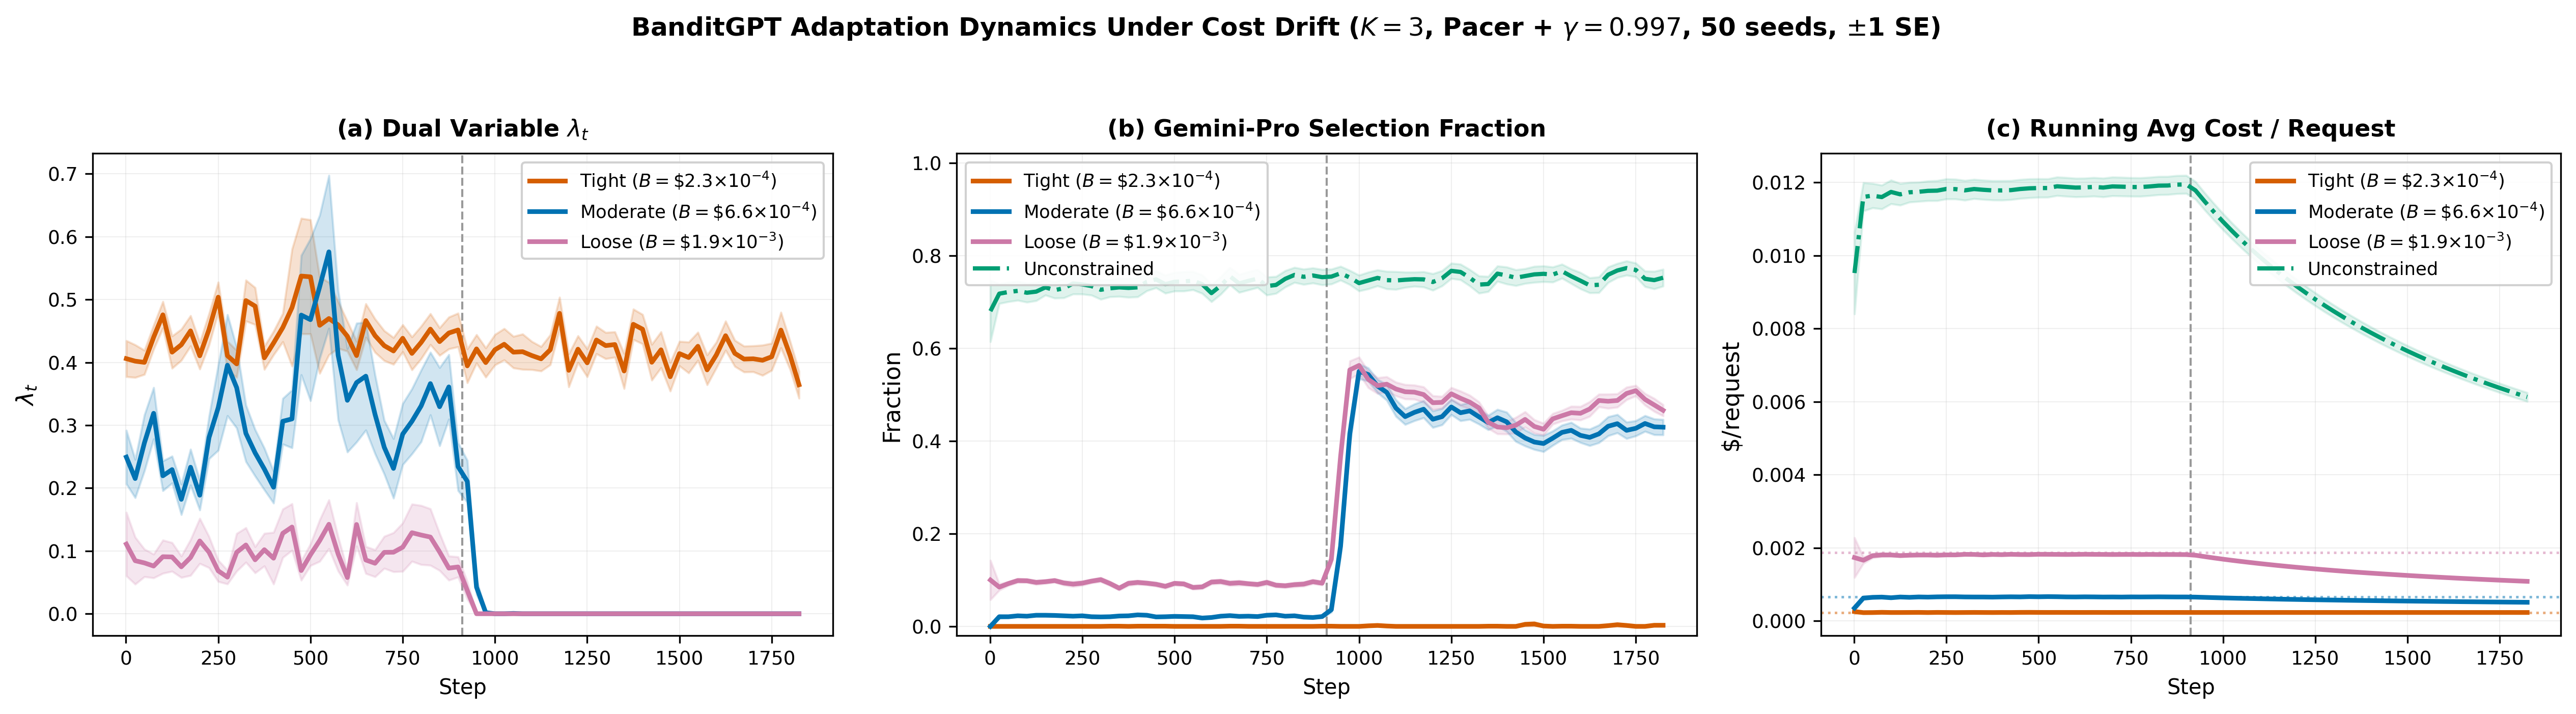
\includegraphics[width=\linewidth]{../experiments/03_budget_plus_drift/results/adaptation_dynamics.pdf}
    \caption{ParetoBandit dual-variable dynamics under a mid-stream
    Gemini price drop (step~912; $K{=}3$, 50~seeds, 95\% bootstrap CI).
    %
    \textbf{(a)}~The dual variable $\lambda_t$ decays at all three
    budget levels after the price drop as costs fall below target;
    the decay is fastest at loose and slowest at tight, where the
    margin is narrowest.
    %
    \textbf{(b)}~Gemini selection fraction surges in Phase~2---tight
    budget reaches ${\sim}68\%$, moderate/loose converge toward the
    unconstrained baseline (dash-dot) at ${\sim}49$--$50\%$.
    %
    \textbf{(c)}~Running average cost per request; dotted lines
    mark budget targets.
    All three regimes exhibit the correct Lagrangian response.
    See Table~\ref{tab:budget_compliance} for quantitative
    compliance comparisons with baselines.
    }
    \label{fig:exp03_adaptation}
\end{figure*}
